% ------------ begin cheatsheet
\documentclass[a4paper]{article}
\usepackage[a4paper,margin=0.15in]{geometry}
\usepackage{multicol}

\usepackage{amsmath, amssymb}
\usepackage[inline]{enumitem}
\usepackage{graphicx}

\usepackage{ulem}
\usepackage{makecell}

% horizontal list
\newlist{hlist}{enumerate*}{1}
\setlist[hlist]{label={}, afterlabel={}, itemjoin={{ \textbar{} }}}

% math
\newcommand{\abs}[1]{\left\lvert#1\right\rvert}
\newcommand{\indep}{\perp \!\!\! \perp}

% envs
\newcommand{\oli}[1]{\begin{enumerate*}[label=(\arabic*)]#1\end{enumerate*}}
\newcommand{\red}[1]{\textcolor{red}{#1}}

\graphicspath{ {./images/} }
\pagestyle{empty}
\setlength{\columnseprule}{0.3pt}

% reduce spacing before and after headers
\newcommand{\uppercaseandunderline}[1]{\uline{\uppercase{#1}}}

\makeatletter
\renewcommand{\section}{
  \@startsection{section}{1}{0pt}{1ex}{1.2ex} {\raggedleft\normalfont\large\bfseries\uppercaseandunderline}}
\renewcommand{\subsection}{
  \@startsection{subsection}{2}{0pt}{1ex}{1.2ex} {\raggedleft\normalfont\normalsize\bfseries\fbox}}
\renewcommand{\subsubsection}{
  \@startsection{subsubsection}{3}{0pt}{1ex}{0.8ex} {\raggedleft\normalfont\small\bfseries\uline}}
\renewcommand{\paragraph}{
  \@startsection{paragraph}{4}{0pt}{1.5ex}{-0.8em}{\normalfont\bfseries}}
% ------------ end cheatsheet

% ------------ begin code
\usepackage{xcolor}
\definecolor{dkgreen}{rgb}{0,0.6,0}
\definecolor{gray}{rgb}{0.5,0.5,0.5}
\definecolor{mauve}{rgb}{0.58,0,0.82}
\definecolor{lg}{rgb}{0.9,0.9,0.9}

% code environment
\usepackage{listings}
\lstset{
  %frame=tb, % adds top and bottom border
  aboveskip=1mm,
  belowskip=1mm,
  showstringspaces=false,
  columns=flexible,
  basicstyle={\small\ttfamily},
  numberstyle=\color{gray},
  keywordstyle=\color{blue}\textbf,
  commentstyle=\color{dkgreen},
  stringstyle=\color{mauve},
  breaklines=true,
  breakatwhitespace=true,
  backgroundcolor=\color{lg},
  tabsize=4
}
\newcommand{\ic}[1]{\lstinline{#1}}

% ------------ end code

\begin{document}
\small
\setlength{\abovedisplayskip}{0pt}
\setlength{\belowdisplayskip}{0pt}
\setlength{\abovedisplayshortskip}{0pt}
\setlength{\belowdisplayshortskip}{0pt}
\begin{multicols*}{2}
  \part*{\centering \underline{CS3230}}
\section*{Intro} 
  \subsection*{Matching problem}
    \begin{itemize}[leftmargin=*]
      \item Input: preference rankings for all $n$ men and $n$ women
      \item Output: a stable matching, where no unmatched man and woman both prefer each other to their current partners
    \end{itemize}
    \subsubsection*{Gale-Shapley (1962)} \noindent
      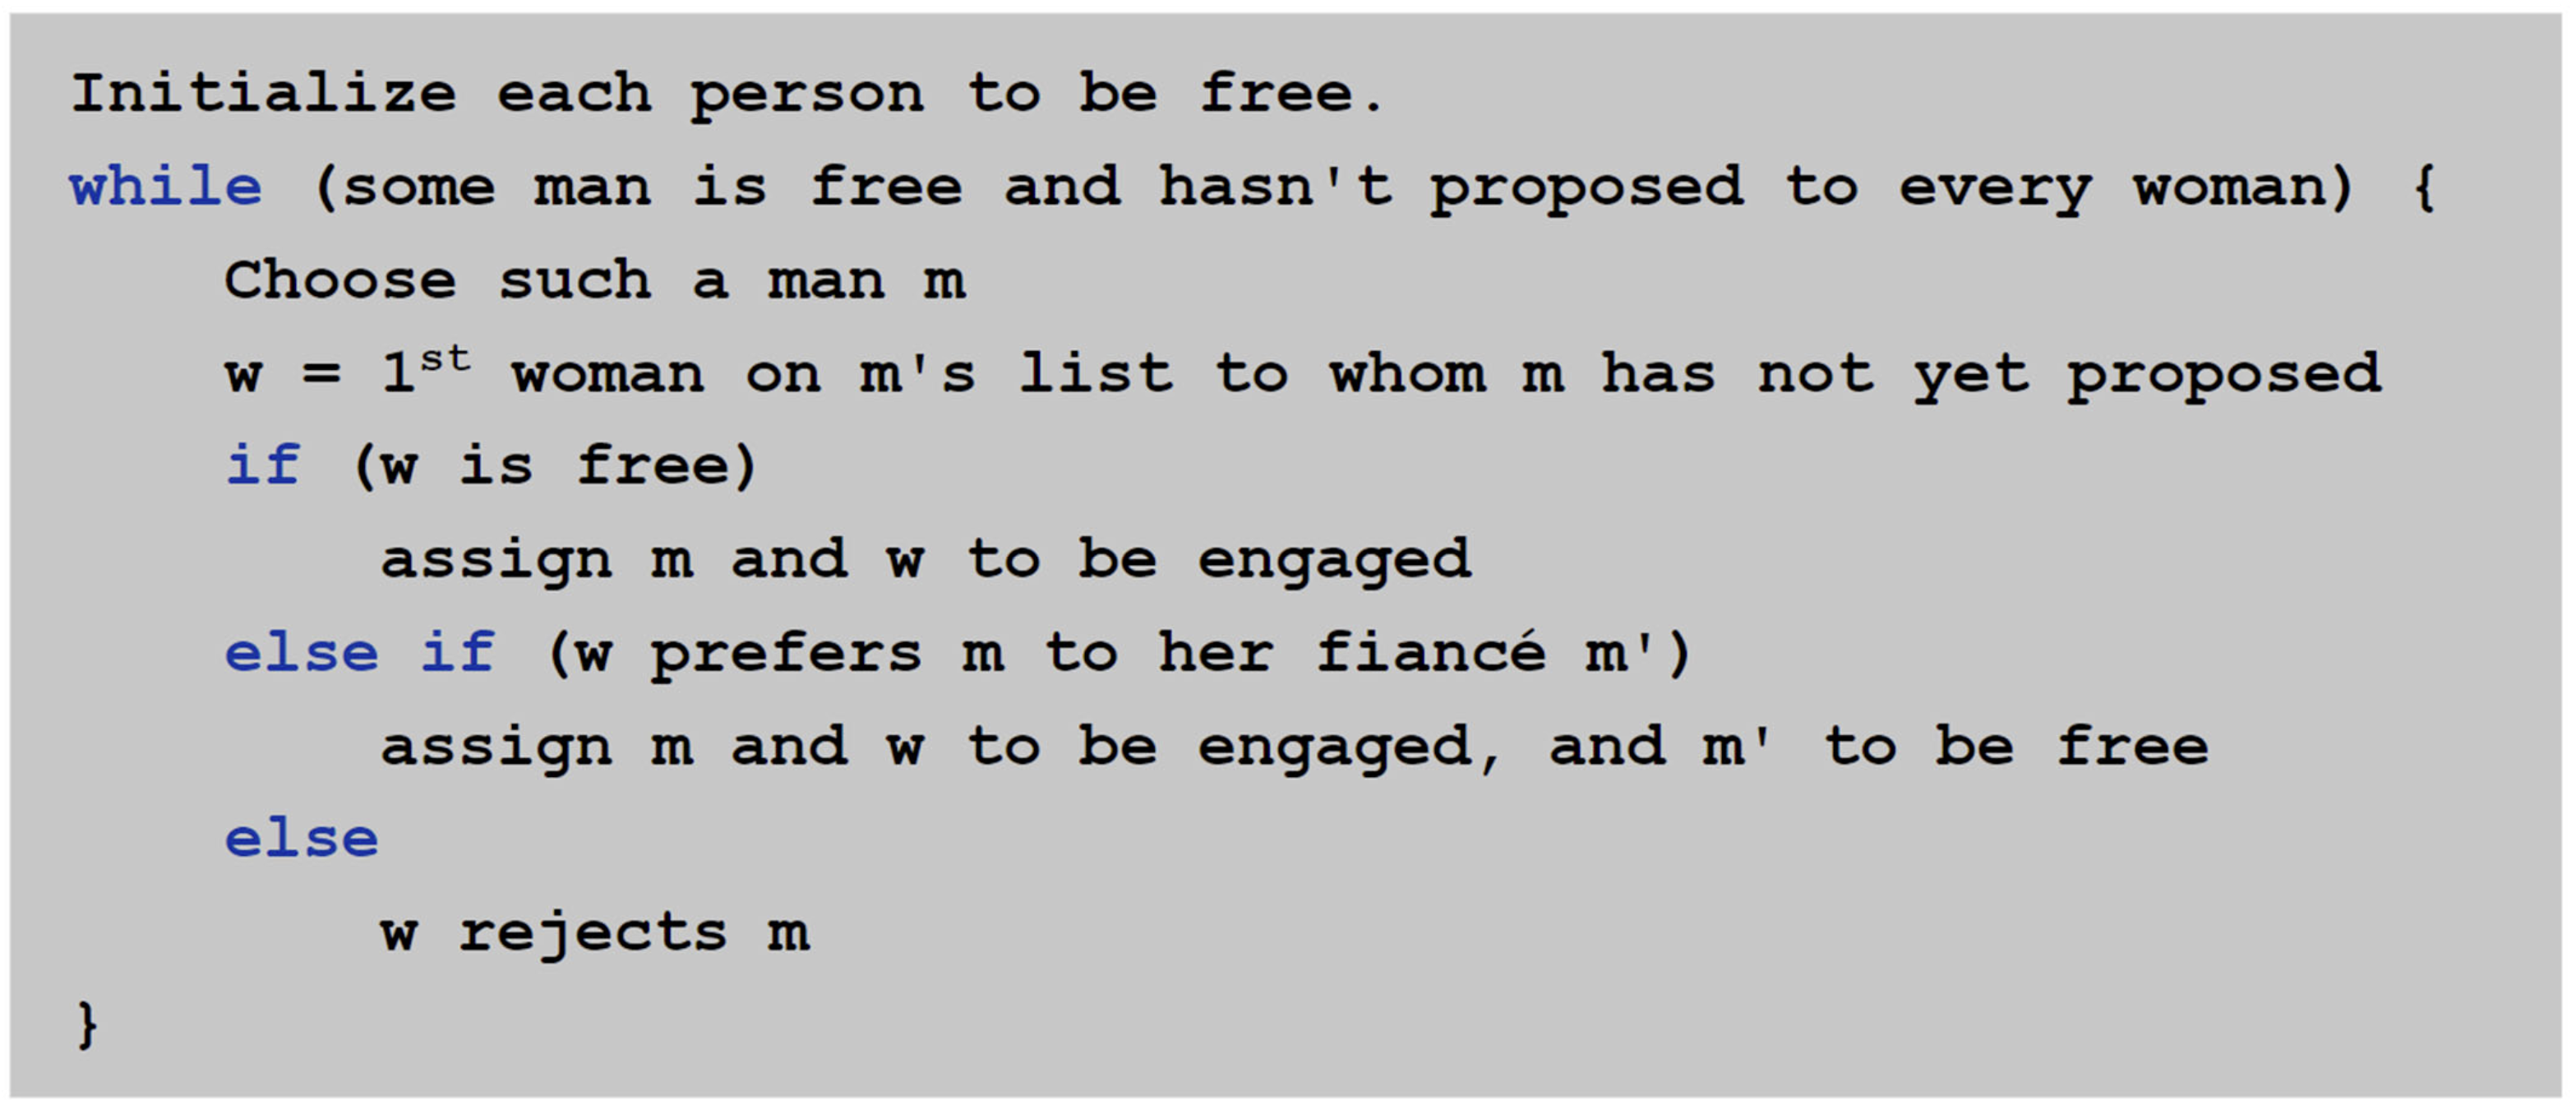
\includegraphics[width=\columnwidth]{gale-shapley}
      \vspace{-0.6cm}
      \paragraph{Properties}
        \begin{itemize}[leftmargin=*]
          \item \ic{while} loop runs $\leq n^2$ times
          \item Men propose to women in decreasing order of preference
          \item A woman stays engaged after the first time she gets engaged. Her sequence of partners keeps getting better according to her preference list
        \end{itemize}
      \paragraph{Properties after terminate}
        \begin{itemize}[leftmargin=*]
          \item Each man is engaged to a unique woman
          \item The matching between men and women is stable
          \item Runs in $O(n^2)$
          \item For a man $m$, let $best(m)$ be the highest ranked woman on his list who could be his partner in some stable matching. Gale-Shapley returns the matching where each man $m$ is paired with $best(m)$.
            \begin{itemize}[leftmargin=*]
              \item No two men have the same optimal partner
              \item All men's wishes are simultaneoulsy optimized
              \item Order of proposals does not matter
            \end{itemize}
          \item In the matching returned by Gale-Shapley, each woman is paired with $worst(w)$.
        \end{itemize}
\section*{Asymptotic analysis}
  \subsection*{Word-RAM model}
    \begin{itemize}[leftmargin=*]
      \item Word is a collection of few bytes
      \item Word is the basic storage unit of RAM, which can be viewed as huge array of words
      \item Each input item is stored in binary format
      \item An arbitrary location of RAM can be accessed in the same time irrespective of the location
      \item Data and program fully reside in RAM
      \item Each arithmetic or logical operation involving a \textbf{constant number} of words takes \textbf{constant number of cycles (steps)} by the CPU
    \end{itemize}
  \subsection*{Big-O notation}
    \paragraph{Upper bound $(\geq)$} \mbox{} \\
      We write $f(n) = O(g(n))$ if for some $c > 0$ and $n_0 > 0$,
      \[ 0 \leq \textbf{f(n)} \leq c g(n) \]
      for all $n \geq n_0$.
    \paragraph{Lower bound $(\leq)$} \mbox{} \\ 
      We write $f(n) = \Omega(g(n))$ if for some $c > 0$ and $n_0 > 0$,
      \[ 0 \leq c g(n) \leq \textbf{f(n)} \]
      for all $n \geq n_0$.
    \paragraph{Tight bound} We write $f(n) = \Theta(g(n))$ if for some positive constants $c_1, c_2, n_0$,
      \[ 0 \leq c_1 g(n) \leq \textbf{f(n)} \leq c_2 g(n) \]
      for all $n \geq n_0$.
    \paragraph{Strict upper bound $(>)$} \mbox{} \\
      We write $f(n) = o(g(n))$ if for some $c > 0$ and $n_0 > 0$,
      \[ 0 \leq \textbf{f(n)} < c g(n) \]
      for all $n \geq n_0$.
    \paragraph{Strict lower bound $(<)$} \mbox{} \\ 
      We write $f(n) = \omega(g(n))$ if for some $c > 0$ and $n_0 > 0$,
      \[ 0 \leq c g(n) < \textbf{f(n)} \]
      for all $n \geq n_0$.
  \subsection*{Properties}
    \subsubsection*{Set notations}
      \begin{itemize}[leftmargin=*]
        \item The notations are really just sets, e.g.
          \begin{align*}
            O(g(n)) =\{& f(n): \exists c > 0, n_0 > 0 \text{ such that} \\
                       & 0 \leq f(n) \leq c(g(n)) \quad \forall n \geq n_0 \}
          \end{align*}
        \item $\Theta(g(n)) = O(g(n)) \cap \Omega(g(n))$
      \end{itemize}
    \subsubsection*{Transitivity} \noindent
      \begin{align*}
        f(n) = \Theta(g(n)) \land g(n) = \Theta(h(n)) & \Rightarrow f(n) = \Theta(h(n)) \\
        f(n) = O(g(n)) \land g(n) = O(h(n)) & \Rightarrow f(n) = O(h(n)) \\
        f(n) = \Omega(g(n)) \land g(n) = \Omega(h(n)) & \Rightarrow f(n) = \Omega(h(n)) \\
        f(n) = o(g(n)) \land g(n) = o(h(n)) & \Rightarrow f(n) = o(h(n)) \\
        f(n) = \omega(g(n)) \land g(n) = \omega(h(n)) & \Rightarrow f(n) = \omega(h(n))
      \end{align*}
    \subsubsection*{Reflexivity} \noindent
      \begin{align*}
        f(n) &= \Theta(f(n)) \\
        f(n) &= O(f(n)) \\
        f(n) &= \Omega(f(n))
      \end{align*}
    \subsubsection*{Symmetry} \noindent
      \[ f(n) = \Theta(g(n)) \iff g(n) = \Theta(f(n)) \]
    \subsubsection*{Complementarity} \noindent
      \begin{align*}
        f(n) = O(g(n)) &\iff g(n) = \Omega(f(n)) \\
        f(n) = o(g(n)) &\iff g(n) = \omega(f(n))
      \end{align*}
  \subsection*{Useful facts}
    \begin{itemize}[leftmargin=*]
      \item Degree-$k$ polynomials are $O(n^k)$, $o(n^{k+1})$, and $\omega(n^{k-1})$
      \item Polynomials dominate logs: 
        \[ (\log n)^{100} = o(n^{.0001}) \]
      \item Exponentials dominate polys:
        \[ n^{1000} = o(2^{.001n}) \]
      \item $\max(f(n), g(n)) = \Theta(f(n) + g(n))$
    \end{itemize}
    \subsubsection*{Exponentials}
      \paragraph{Misc}
        \begin{itemize}[leftmargin=*]
          \item For constants $k>0, a>1, n^k = o(a^n)$
          \item Exponentials of different bases differ by an \textbf{exponential factor}
          \item $2^{n+5} = O(2^n)$, but $2^{5n} \neq O(2^n)$
        \end{itemize}
      \paragraph{Properties} \mbox{} \\
        \begin{minipage}{.475 \columnwidth}
          \begin{align*}
            a^{-1} &= \frac{1}{a} \\
            (a^m)^n &= a^{mn}
          \end{align*}
        \end{minipage}
        \begin{minipage}{.475 \columnwidth}
          \begin{align*}
            a^m a^n &= a^{m+n} \\
            e^x &\geq 1 + x
          \end{align*}
        \end{minipage}
    \subsubsection*{Logarithms}
      \paragraph{Types} \mbox{} \\
        \begin{minipage}{.45 \columnwidth}
          \begin{itemize}[leftmargin=*]
            \item Binary log: $\lg n = \log_2 n$
            \item Natural log: $\ln n = \log_e n$
          \end{itemize}
        \end{minipage}
        \begin{minipage}{.525 \columnwidth}
          \begin{itemize}[leftmargin=*]
            \item Exponentiation: $\lg^k n = (\lg n)^k$
            \item Composition: $\lg \lg n = \lg (\lg n)$
          \end{itemize}
        \end{minipage}
      \paragraph{Misc}
        \begin{itemize}[leftmargin=*]
          \item Base of log does not matter in asymptotics
            \[ \lg n = \Theta(\ln n) = \Theta(\log_{10} n) \]
        \end{itemize}
      \paragraph{Properties} \mbox{} \\
        \begin{minipage}{.475 \columnwidth}
          \begin{align*}
            a &= b^{\log_b a} \\
            \log_c(ab) &= \log_c a + \log_c b \\
            \log_b a^n &= n \log_b a \\
            \log_b a &= \frac{\log_c a}{\log_c b}
          \end{align*}
        \end{minipage}
        \begin{minipage}{.475 \columnwidth}
          \begin{align*}
            \log_b \frac{1}{a} &= - \log_b a \\
            \log_b a &= \frac{1}{\log_a b} \\
            a^{\log_b c} &= c^{\log_b a}
          \end{align*}
        \end{minipage}
    \subsubsection*{Overview} \noindent
      \[ 1 < \log n < \sqrt{n} < n < n \log n < n^2 < n^3 < 2^n < 2^{2n} < n! < n^n \]
  \subsection*{Misc}
    \paragraph{Stirling's approximation}
      \begin{align*}
        n! &= \sqrt{2 \pi n} \left(\dfrac{n}{e}\right)^n \left(1 + \Theta\left(\frac{1}{n}\right)\right) \\
        \log(n!) &= \Theta(n \lg n)
      \end{align*}
    \paragraph{Arithmetic series}
      \[ \sum_{k=1}^n k = \frac{n(n+1)}{2} = \Theta(n^2) \]
    \paragraph{Geometric series}
      \begin{align*}
        \sum_{k=0}^n x^k &= \frac{x^{n+1} - 1}{x - 1} \\
        \sum_{k=0}^\infty x^k &= \frac{1}{1-x} \text{ when } \lvert x \rvert < 1
      \end{align*}
    \paragraph{Harmonic series}
      \[ \sum_{k=1}^\infty \frac{1}{k} = \ln n + O(1) \]
  \subsection*{Limits} \noindent
    Assume $f(n), g(n) > 0$.
    \begin{align*}
      \lim_{n \rightarrow \infty} \frac{f(n)}{g(n)} = 0 &\Rightarrow f(n) = o(g(n)) \\
      \lim_{n \rightarrow \infty} \frac{f(n)}{g(n)} < \infty &\Rightarrow f(n) = O(g(n)) \\
      0 < \lim_{n \rightarrow \infty} \frac{f(n)}{g(n)} < \infty &\Rightarrow f(n) = \Theta(g(n)) \\
      \lim_{n \rightarrow \infty} \frac{f(n)}{g(n)} > 0 &\Rightarrow f(n) = \Omega(g(n)) \\
      \lim_{n \rightarrow \infty} \frac{f(n)}{g(n)} = \infty &\Rightarrow f(n) = \omega(g(n)) \\
    \end{align*}
    \paragraph{Epsilon-delta definition}
      Let $f(x)$ be a function defined on an open interval around $x_0$, where $f(x_0)$ need not be defined. Then
      \[ \lim_{x \rightarrow x_0} f(x) = L \]
      if for every $\varepsilon$ there exists $\delta > 0$ such that for all $x$,
      \[ 0 < \lvert x - x_0 \rvert < \delta \implies \lvert f(x) - L \rvert < \varepsilon \]
    \paragraph{L'Hopital}
      If $\lim_{x \rightarrow \infty} f(x) = \lim_{x \rightarrow \infty} g(x) = 0 \text{ or } \pm \infty$,
      \[ \lim_{x \rightarrow \infty} \frac{f(x)}{g(x)} = \lim_{x \rightarrow \infty} \frac{f'(x)}{g'(x)} \]
\section*{Correctness}
  \subsection*{Iterative algorithms}
    \subsubsection*{Loop invariant}
      \begin{itemize}[leftmargin=*]
        \item True at the beginning of an iteration
        \item Remains true at beginning of next iteration
        \item If still true at end, then it implies algorithm's correctness
      \end{itemize}
    \subsubsection*{Showing correctness}
      \begin{itemize}[leftmargin=*]
        \item Initialization: Invariant is true before first iteration
        \item Maintenance: If invariant is true before an iteration, it remains true before the next iteration
        \item Termination: When the algorithm terminates, the invariant provides a useful property for showing correctness
      \end{itemize}
  \subsection*{Recursive algorithms} \noindent
    Express time complexity in terms of recurrence:
    \[ T(n) = a T\left(\frac{n}{b}\right) + f(n) \]
    \subsubsection*{Recursion tree} \noindent
      Draw tree of problem being recursively broken down, where the value at each node is the cost for that node. Sum up all costs to get the overall time complexity. \\
      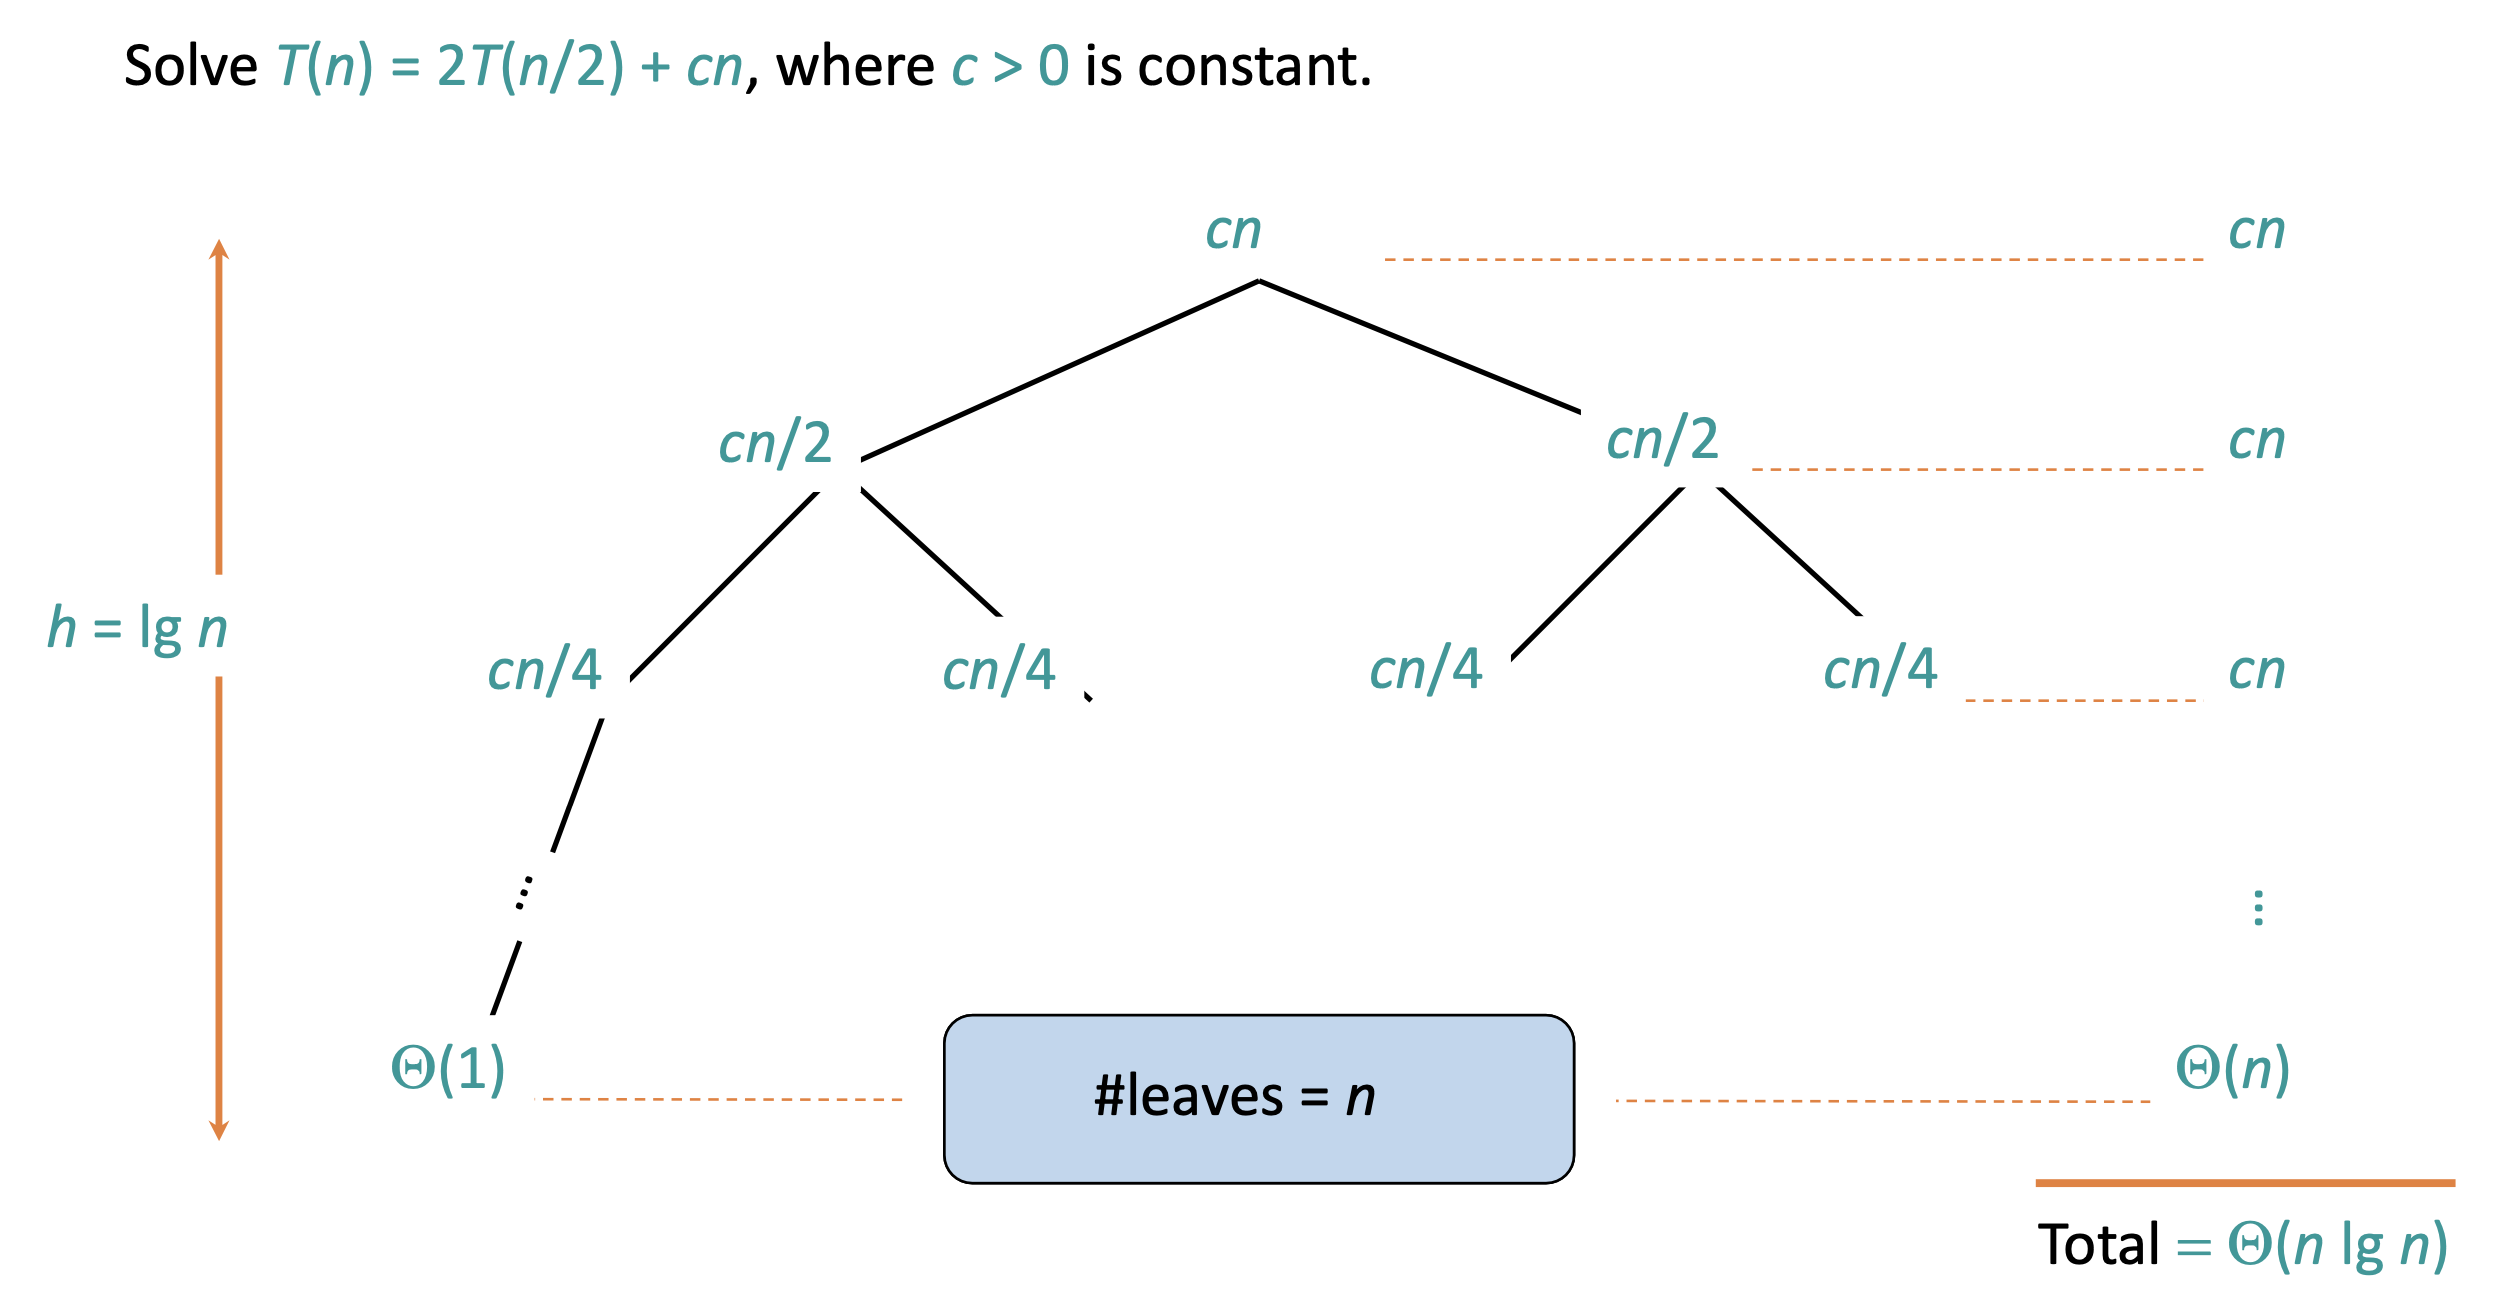
\includegraphics[width=0.9\columnwidth]{recursion-tree}
      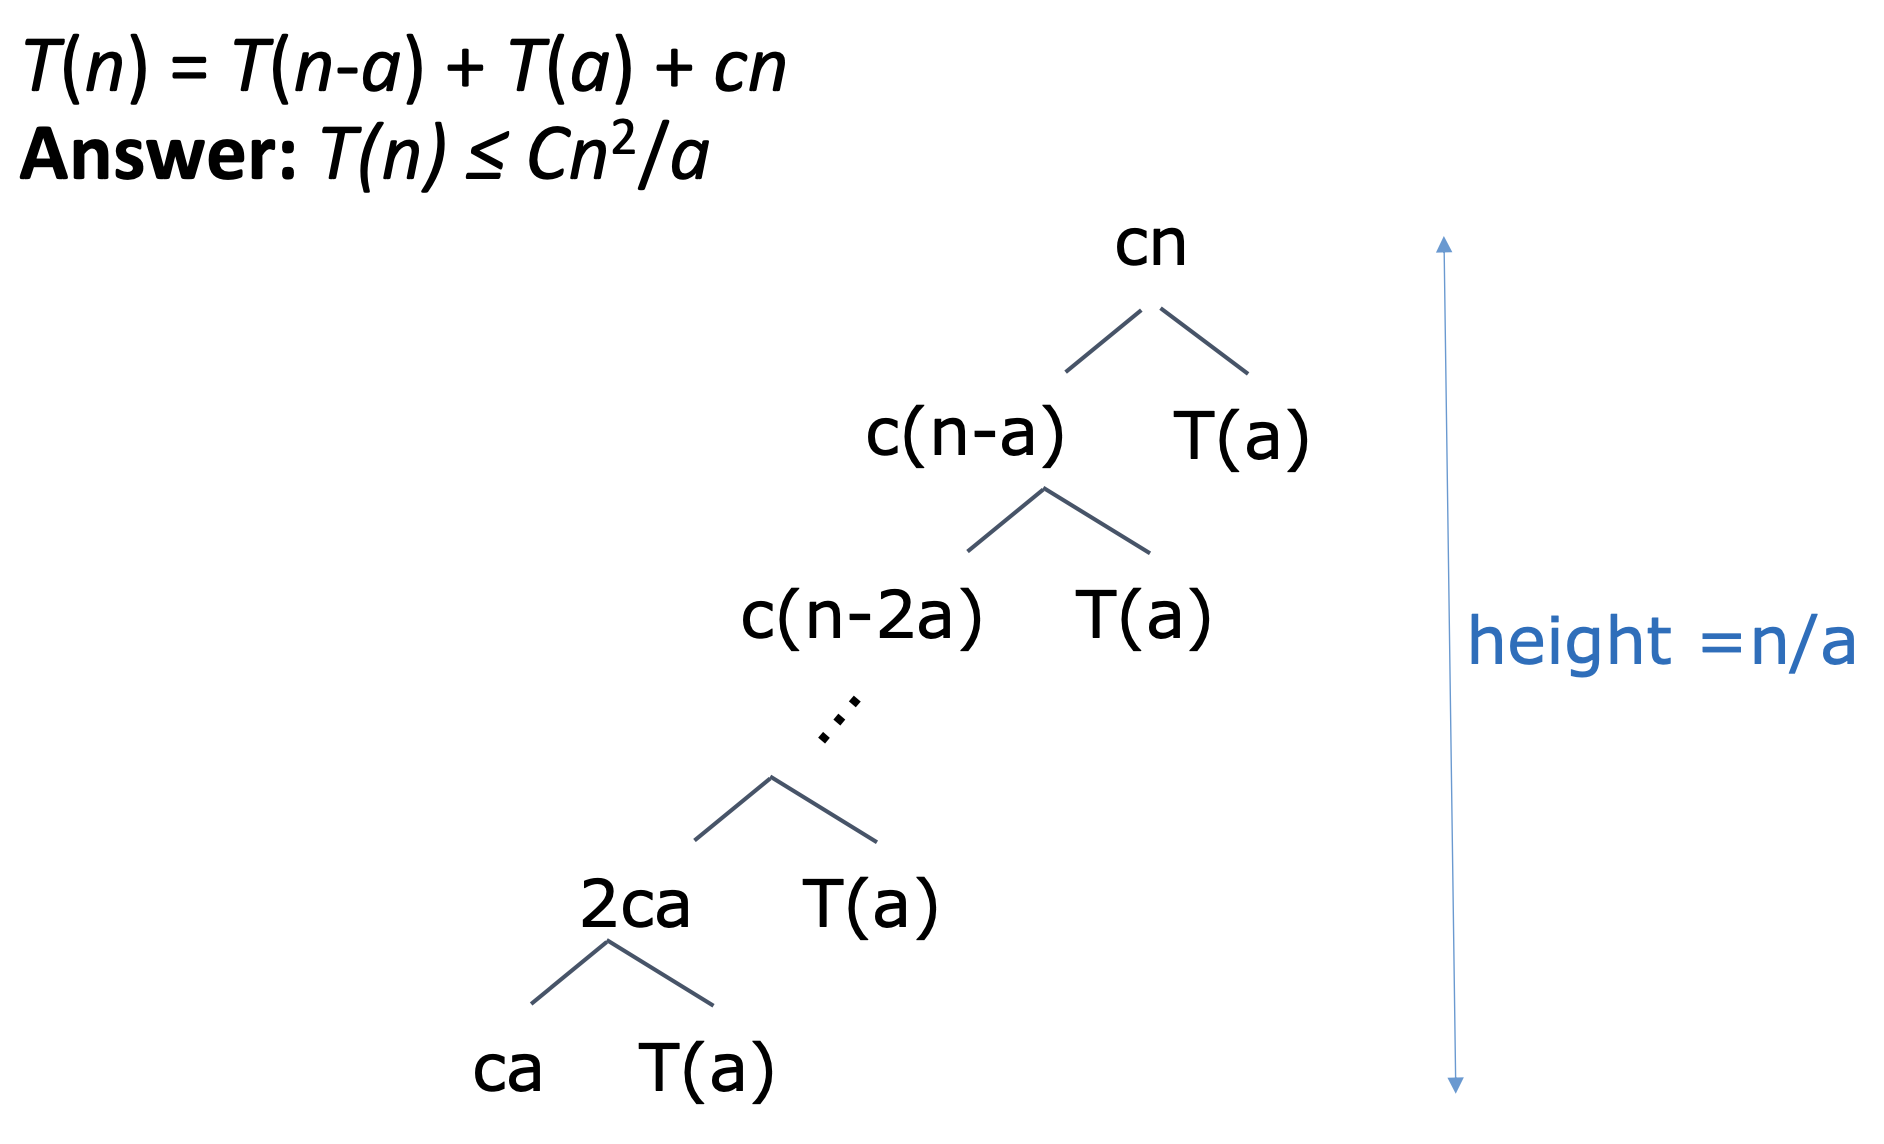
\includegraphics[width=0.9\columnwidth]{recursion-tree-2}
    \subsubsection*{Master method} \noindent
      Comparing $f(n)$ with $n^{\log_b(a)}$ as polynomials, for $a \geq 1, b > 1, k \geq 0, \epsilon > 0$ and $f$ is asymptotically positive,
      \begin{align*}
        T(n) &= a T\left( \frac{n}{b} \right) + f(n) \\
        &= \begin{cases}
             \Theta(n^{\log_b(a)}) & \text{if } f(n) = O(n^{\log_b(a) - \epsilon}) \\
             \Theta(n^{\log_b(a)} \log^{k+1} n) & \text{if } f(n) = \Theta(n^{\log_b(a)} \log^k n) \\
             \Theta(f(n)) & \text{if } f(n) = \Omega(n^{\log_b(a) + \epsilon})
           \end{cases}
      \end{align*}
      For case 3, $f(n)$ must satisfy the regularity condition that $a f(n/b) \leq c f(n)$ for some $c < 1$, which guarantees that the sum of subproblems is smaller than $f(n)$. But this is typically satisified anyway.
    \subsubsection*{Substitution method}
      \begin{itemize}[leftmargin=*]
        \item Guess the form of the solution
        \item Verify by induction
      \end{itemize}
  \subsection*{Exponentiation}
    \begin{itemize}[leftmargin=*]
      \item Divide: Trivial
      \item Conquer: Recursively compute $f(\lfloor n/2 \rfloor, m)$
      \item Combine:
        \begin{itemize}[leftmargin=*]
          \item $f(n,m) = f(\lfloor n/2 \rfloor, m)^2 (\text{mod } m)$ if $n$ is even;
          \item $f(n,m) = f(1, m) \cdot f(\lfloor n/2 \rfloor, m)^2 (\text{mod } m)$ if $n$ is odd
        \end{itemize}
      \item $T(n) = T(n/2) + \Theta(1)$, so by master theorem, we have $T(n) = \Theta(\lg n)$
    \end{itemize}
  \subsection*{Induction}
    \begin{itemize}[leftmargin=*]
      \item Verify base case
      \item Show that if the statement is true for the $k$th case (regular induction) or all cases up to the $k$th case (strong induction) , then it is also true for the $(k+1)$th case
      \item Conclude that the statement is true for all cases
    \end{itemize}
\section*{Randomized algos}
  \subsection*{Probability}
    \subsubsection*{Axioms} \noindent
      Let $S$ be a set (the full sample space). A function $P$ is called probability if it assigns values to each subset of $S$, subject to:
      \begin{itemize}[leftmargin=*]
        \item $\forall A \subset S, 0 \leq P(A) \leq 1$
        \item $P(S) = 1$
        \item If $A_1, A_2, \cdots$ are disjoint subsets of $S$, then $P(A_1 + A_2 + \cdots) = P(A_1) + P(A_2) + \cdots$
      \end{itemize}
      \paragraph{Results}
        \begin{itemize}[leftmargin=*]
          \item $P(\emptyset) = 0$
          \item For $A \subset S$, let $A^C$ be the complement of $A$, then $P(A^C) = 1 - P(A)$
          \item Let $A \subset B \subset S$, then $P(A) \leq P(B)$
        \end{itemize}
    \subsubsection*{Conditional probability} \noindent
      Let $A$ and $B$ be events in a sample space $S$. If $P(A) \neq 0$, then the conditional probability of $B$ given $A$ is
      \[ P(B \;\vert\; A) = \dfrac{P(A \cap B)}{P(A)} = \dfrac{P(A \;\vert\; B)P(B)}{P(A)} \]
      If we do not have $P(A)$, then we have to calculate it using disjoint events:
      \[
        P(B_k \;\vert\; A) = \dfrac{P(A \;\vert\; B_k) P(B_k)}{P(A \;\vert\; B_1) P(B_1) + \cdots + P(A \;\vert\; B_n) P(B_n)}
      \]
    \subsubsection*{Independence} \noindent
      Definition:
      \[ P(A \cap B) = P(A) P(B \;\vert\; A) = P(A)P(B) \]
      We may use $A \indep B$ to mean $A$ and $B$ are independent. When $A \indep B$,
      \begin{itemize}[leftmargin=*]
        \item $A^C \indep B, A \indep B^C, A^C \indep B^C$
        \item If $P(A) > 0$, then $P(B \;\vert\; A) = P(B)$
        \item If $P(B) > 0$, then $P(A \;\vert\; B) = P(A)$
      \end{itemize}
      \paragraph{Joint (Mutual) independence}
        3 events $A,B,C$ are jointly independent if
        \begin{itemize}[leftmargin=*]
          \item $A, B, C$ pairwise indepdent
          \item $P(A \cap B \cap C) = P(A)P(B)P(C)$
        \end{itemize}
    \subsubsection*{Expectation} \noindent
      Let $X$ be a discrete random variable taking values in $\mathbb{Z}$. Let $x_i$ denote the possible realizations of $X$. The expected value of $X$ is
      \[ E(X) = \sum_{x_i \in \mathbb{Z}} x_i P(X = x_i) \]
      \paragraph{Properties}
        \begin{itemize}[leftmargin=*]
          \item $E(a) = a$ for real constant $a$
          \item $E(aX+b) = aE(X) + b$ for real constants $a, b$
          \item If $A$ and $B$ are indepdent, $E(AB) = E(A) E(B)$
        \end{itemize}
      \paragraph{Linearity of expectation} \noindent
        For random variables $X$ and $Y$:
        \[ E(aX + bY) = a E(X) + b E(Y) \]
    \subsubsection*{Indicator Random Variables} \noindent
      Let $X$ be a indicator random variable associated with an event $A$, that occurs with probability $p$:
      \[ X = \begin{cases}
        1 & \text{with probability } p \\
        0 & \text{with probability } 1-p
      \end{cases} \]
      Then $E(X) = p$.
    \subsubsection*{Bernoulli trials} \noindent
      \begin{itemize}[leftmargin=*]
        \item A Bernoulli trial is an experiment that has probability $p$ of success, and probability $q = 1-p$ of failure
        \item Let $X$ be the number of Bernoulli trials before the first success
          \[ \mathrm{Pr}[ X=k ] = (1-p)^{k-1} \cdot p \]
          and this is a geometric distribution, with $E[X] = \frac{1}{p}$
      \end{itemize}
  \subsection*{Quick sort}
    \begin{itemize}[leftmargin=*]
      \item Worst case: $O(n^2)$
      \item Average case, select 1st element as pivot: $O(n \log n)$
        \begin{itemize}[leftmargin=*]
          \item Depends on initial input permutation
        \end{itemize}
      \item Outperforms merge sort, because
        \begin{itemize}[leftmargin=*]
          \item Less overhead of temporary storage
          \item Fewer cache misses
        \end{itemize}
      \item Worst case expected, with random pivot: $O(n \log n)$
      \item Randomized quick select: $O(n)$
    \end{itemize}
    \subsubsection*{Randomized analysis}
      \begin{itemize}[leftmargin=*]
        \item Select pivots uniformly at random
        \item Time taken depends on random choice of pivot, rather than randomness of input
      \end{itemize}
  \subsection*{Types of randomized algorithms}
    \subsubsection*{Randomized Las Vegas algorithms}
      \begin{itemize}[leftmargin=*]
        \item Output is always correct
        \item Running time is a random variable
      \end{itemize}
    \subsubsection*{Randmoized Monte Carlo algorithms}
      \begin{itemize}[leftmargin=*]
        \item Output may be incorrect with some small probability
        \item Running time is deterministic
      \end{itemize}
\section*{Hashing}
  \subsection*{Dictionary}
    \begin{itemize}[leftmargin=*]
      \item Maintains (key, value) pairs
      \item Inserting a key will overwrite the value
      \item Querying a key will return the value
    \end{itemize}
    \paragraph{Variants}
      \begin{itemize}[leftmargin=*]
        \item Static: Inserted items are fixed, only care about queries
        \item Insertion-only: Only insertions and queries
        \item Dynamic: Insertions, deletions, queries
      \end{itemize}
    \paragraph{Implementation}
      \begin{itemize}[leftmargin=*]
        \item Static: sorted list - $O(\log n)$ queries
        \item Dynamic: balanced search tree - $O(\log n)$ operations
      \end{itemize}
  \subsection*{Hashing}
    \paragraph{Desired properties}
      \begin{itemize}[leftmargin=*]
        \item Minimize collisions
        \item Minimize storage space $M$, aim is $M = O(N)$
        \item Hash function should be easy to compute. Assume that hash can be computed in constant time
      \end{itemize}
  \subsection*{Universal hashing} \noindent
    Suppose $\mathcal{H}$ is a set of hash functions mapping $U$ to $[M]$. We say $\mathcal{H}$ is universal if for all $x \neq y$,
    \[ \frac{\lvert h \in \mathcal{H}: h(x) = h(y) \rvert}{\lvert\mathcal{H}\rvert} \leq \frac{1}{M} \]
    or, using probability,
    \[ \underset{h \sim \mathcal{H}}{\mathrm{Pr}} [h(x) = h(y)] \leq \frac{1}{M} \]
    \begin{itemize}[leftmargin=*]
      \item i.e. For any $x \neq y$, if $h$ is chosen uniformly at random from universe $\mathcal{H}$, there's at most $\frac{1}{M}$ probability that $h(x) = h(y)$.
      \item Note: hash function is \textbf{fixed} throughout the lifetime of the dictionary, unless otherwise stated
      \item Consider the table below. For a hash function $h$ drawn from a universal hash family, the above inequality states that the sum along the highlighted diagonal is $\leq \dfrac{1}{M}$.
    \end{itemize}
    \vspace{-0.2cm}
    \begin{center}
      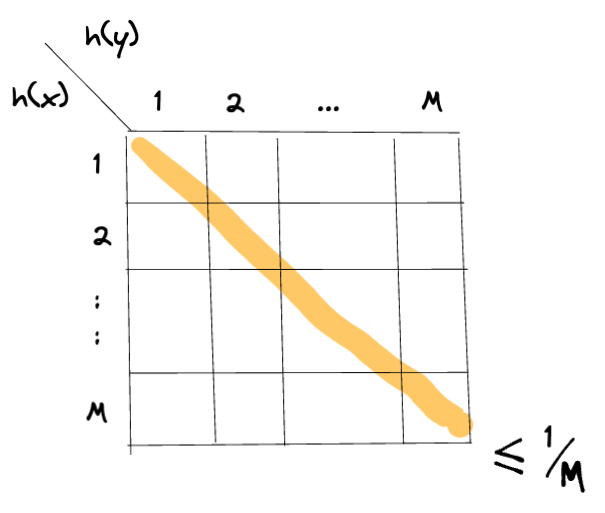
\includegraphics[width=0.5\columnwidth]{universal-hashing}
    \end{center}
    \subsubsection*{Properties} \noindent
      \begin{itemize}[leftmargin=*]
        \item For any $N$ elements $x_1, x_2, \cdots, x_N$, the expected number of collisions between $x_N$ and the other elements is $\frac{N-1}{M}$ which is less than $\frac{N}{M}$.
          \begin{itemize}[leftmargin=*]
            \item i.e. the cost of an operation is $O(1)$
          \end{itemize}
        \item For any sequence of $N$ insertions, deletions and queries, if $M \geq N$, then the expected total cost for a random $h \in \mathcal{H}$ is $O(N)$
      \end{itemize}
    \subsubsection*{Construction} \noindent
      Suppose $U$ is indexed by $u$-bit strings, and $M = 2^m$. For any binary matrix $A$ with $m$ rows and $u$ columns,
      \[ h_A(x) = Ax \; (\text{mod } 2) \]
      where $x \in U$ is a column vector. Then the hash family
      \[ \{ h_A: A \in \{0, 1\}^{m \times u} \} \]
      is universal.
      \paragraph{Additional storage}
        \begin{itemize}[leftmargin=*]
          \item Has overhead of $\Theta(\log N \cdot \log U)$ bits if $M = \Theta(N)$
        \end{itemize}
  \subsection*{Uniform hashing} \noindent
    $\mathcal{H}$ is said to be a uniform family of hash functions if for every key $x \in U$ and every hash value $i \in [M]$, it holds that
    \[ \underset{h \leftarrow \mathcal{H}}{\mathrm{Pr}} [h(x) = i] \leq \frac{1}{M} \]
  \subsection*{Pairwise independent} \noindent
    $\mathcal{H}$ is pairwise independent, if for any two distinct $x, y \in U$, and for any two hash values $i_1, i_2$
    \[ \underset{h \sim \mathcal{H}}{\mathrm{Pr}} [h(x) = i_1, h(y) = i_2] = \frac{1}{M^2} \]
    \begin{itemize}[leftmargin=*]
      \item Pariwise independent $\Rightarrow$ Universal, but not the converse.
    \end{itemize}
    Consider the table below. For a hash function $h$ drawn from a pairwise independent hash family, the above equality states that the probability in each cell is exactly $\dfrac{1}{M^2}$.
    \vspace{-0.2cm}
    \begin{center}
      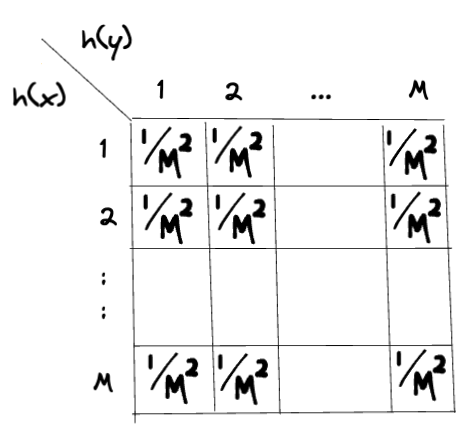
\includegraphics[width=0.5\columnwidth]{pairwise-independent-hashing}
    \end{center}
  \subsection*{(Static) perfect hashing} \noindent
    \begin{itemize}[leftmargin=*]
      \item Want to do all queries in worst-case constant time
    \end{itemize}
    \subsubsection*{Using quadratic space} \noindent
      If $\mathcal{H}$ is universal, and $M = N^2$, then if $h$ is sampled uniformly from $\mathcal{H}$, the expected number of collisions is $< 1$.
      \begin{itemize}[leftmargin=*]
        \item For $i \neq j$, let $A_{ij} = 1$ if $h(x_i) = h(x_j)$, 0 otherwise
        \item By universality, $E[A_{ij}] = \mathrm{Pr}[A_{ij} = 1] \leq \frac{1}{M} = \frac{1}{N^2}$
        \item $E[\text{collisions}] = \sum_{i \neq j} E[A_{ij}] \leq \binom{n}{2} \frac{1}{N^2} < 1$
      \end{itemize}
    \subsubsection*{2-level scheme}
      \begin{itemize}[leftmargin=*]
        \item Choose $h: U \mapsto [N]$ from a universal hash family
        \item Let $L_k$ be the number of $x_i$ for which $h(x_i) = k$
        \item Choose $h_1, \cdots, h_N$ second-level functions $h_k: [N] \mapsto [L_k^2]$ for each hash value $k$, such that there are no collisions among the $L_k$ elements mapped to $k$ by $h$
          \begin{itemize}[leftmargin=*]
            \item Such a hash function exists because of the quadratic space example earlier
          \end{itemize}
        \item Space used is $O(N)$ (for first level) and $E[ \sum_k L_k^2 ] = O(N)$ (for second level)
      \end{itemize}
      \paragraph{Proof}
        \begin{itemize}[leftmargin=*]
          \item For $1 \leq i, j \leq N$, define $A_{ij} = 1$ if $h(x_i) = h(x_j)$ and $A_{ij} = 0$ otherwise
          \item Note that $\sum_k L_k^2 = \sum_{i,j} A_{ij}$
            \begin{align*}
              E[\sum_{ij} A_ij] &= \sum_i E[A_{ii}] + \sum_{i \neq j} E[A_{ij}] \\
                                &\leq N \cdot 1 + N(N-1) \cdot \frac{1}{N} \\
                                &< 2N
            \end{align*}
        \end{itemize}
\section*{Amortized analysis} \noindent
  Guarantees the average performance of each op in the worst case 
  \subsection*{Aggregate method}
    \begin{itemize}[leftmargin=*]
      \item Count total cost and divide by number of operations
    \end{itemize}
    \subsubsection*{Queues}
      \begin{itemize}[leftmargin=*]
        \item $n$ INSERT and EMPTY operations
        \item Notice EMPTY is a sequence of DELETES, and DELETES $\leq$ INSERTS
        \item If there are $k$ INSERTs, then sum of cost of all EMPTYs is $\leq k$
        \item Total cost $\leq k + k = 2k \leq 2n$ since $k \leq n$. Amortized cost is $O(1)$
      \end{itemize}
  \subsection*{Accounting method}
    \begin{itemize}[leftmargin=*]
      \item Charge $i$th operation a fictitious amoritzed cost $c(i)$, that satisfies
        \[ \sum_{i=1}^n t(i) \leq \sum_{i=1}^n c(i) \quad \forall n \]
        where $t(i)$ is the true cost of the $i$th operation
      \item Usually $c(i) > t(i)$, with the extra amount paid stored as credit for future, rare, expensive operations
      \item Analysis should ensure that there's always enough credit to pay for ture cost
      \item Always \textbf{identify the expensive operation}, which you try to do ``free of cost'' using stored credit
    \end{itemize}
    \subsubsection*{Queues}
      \begin{itemize}[leftmargin=*]
        \item For INSERT, set amortized cost to 2 (true cost is 1)
        \item For EMPTY, set amortized cost to 0 (true cost is size of queue)
        \item Whenever an element is inserted, we pay an extra 1. This extra 1 can be used as credit to pay for later deletions
        \item Total cost is at most $2 \; \times$ number of INSERTS $\leq 2n$
      \end{itemize}
    \subsubsection*{Binary increment}
      \begin{itemize}[leftmargin=*]
        \item Charge 2 for each $0 \rightarrow 1$; Charge 0 for each $1 \rightarrow 0$
        \item Starting from 0, actual cost for $n$ increments is $O(n)$
      \end{itemize}
  \subsection*{Potential method}
    \subsubsection*{Motivation}
      \begin{itemize}[leftmargin=*]
        \item Accounting method tries to eyepower the required amortized cost
        \item Potential method tries to find some metric that decreases a lot on expensive operations
        \item Similar idea
      \end{itemize}
    \subsubsection*{Idea}
      \begin{itemize}[leftmargin=*]
        \item Define potential function $\phi$, where $\phi(i)$ denotes potential at the end of the $i$th operation
        \item Must have $\phi(i) \geq 0$ for all $i$
        \item Amortized cost of $i$th operation, $c(i)$ is defined as
          \[ c(i) = t(i) + \phi(i) - \phi(i-1) \]
        \item Amortized cost of $n$th operations
          \[
            \sum_i c(i) = \sum_i t(i) + (\phi(n) - \phi(0)) \geq \sum_i t(i) - \phi(0)
          \]
        \item Select suitable $\phi$ so that for the \textbf{costly} operation, $\Delta \phi_i$ is \textbf{negative to an extent} that it nullifies or reduces the effect of the actual cost
      \end{itemize}
    \subsubsection*{Binary increment}
      \paragraph{Working}
        \begin{itemize}[leftmargin=*]
          \item Use $\phi(i) = $ number of 1s in the counter after $i$th increment
          \item Let $L_i$ be the length of the longest suffix with all 1s
          \item True cost of $i$th increment is $1 + L_i$
          \item $\Delta \phi_i = -L_i + 1$
          \item Sum of actual cost and $\Delta \phi_i$ is 2, so amortized cost of $i$th increment is 2
        \end{itemize}
      \paragraph{Results}
        \begin{itemize}[leftmargin=*]
          \item Starting from 0, actual cost for $n$ increments is $O(n)$
          \item Starting from $t$ ones, actual cost for $n$ increments is $O(n+t)$
        \end{itemize}
\section*{Misc}
  \subsection*{Inversion} \noindent
    Given an array of integers, the pair $(i,j)$ is called an inversion if $i < j$ and $A[i] > A[j]$
\end{multicols*}
\end{document}
